\chapter{CSP Models for Puzzle Games}
\label{cha:design}
Generally, this chapter discusses two parts: the 2D game (IQ twist) and the 3D game (ZIG ZAG Puzzler). For both games, their CSP models and implementations will be introduced.
\section{IQ Twist}
IQ twist is a puzzle game which consists of 8 twisted puzzle pieces and 7 coloured pegs (Figure~\ref{fig:IQ_twist_game}). To play the game, the colored pegs should be placed on the board, then fit all the twisted puzzle pieces back into the board. Different units of pieces must match the pegs with the same color and only the hollow units of piece can be used to match pegs. The degree of difficulty can be adjusted by the placements of pegs.
\begin{figure}[htbp]
    \centering
    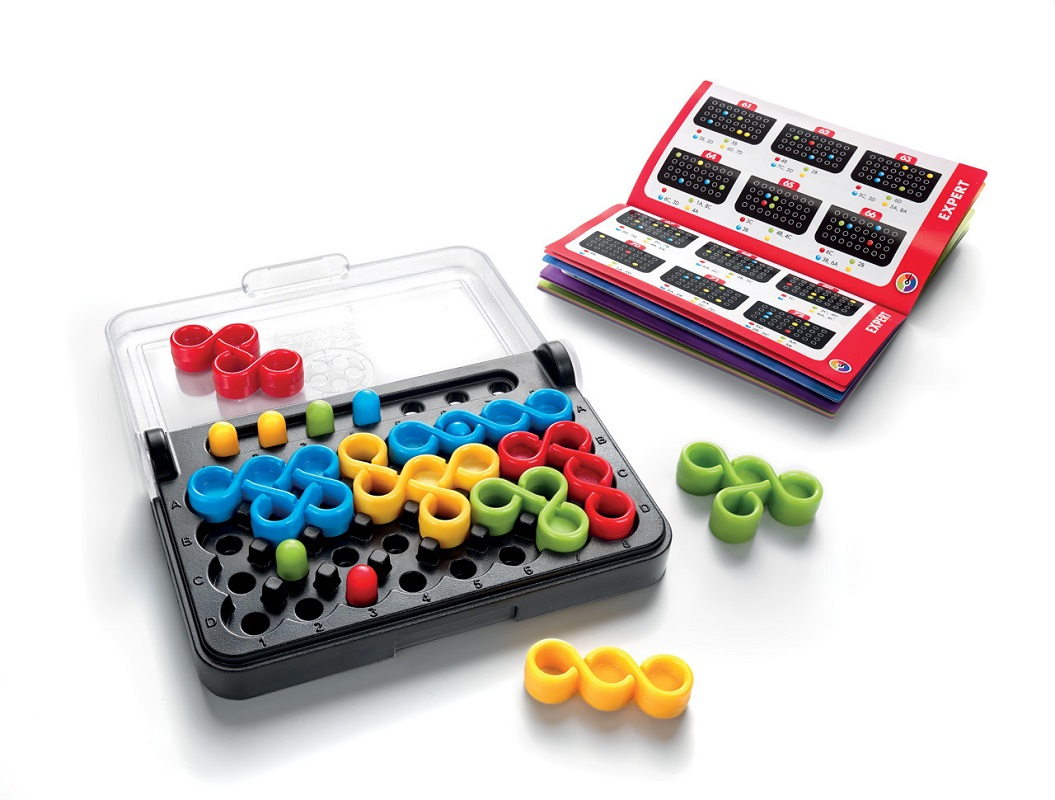
\includegraphics[width=0.5\textwidth]{figs/IQtwistintroduction.jpg}
    \caption{IQ twist game}
    \label{fig:IQ_twist_game}
\end{figure}
\subsection{Variables}
Above all, the initial state of each piece is defined in Figure~\ref{fig:allinit}.
\begin{figure}[htbp]
\begin{subfigure}[b]{.24\textwidth}
\centering

\includegraphics[width=0.75\textwidth]{figs/yellow1.jpg}
\caption{Initial state of yellow1}
  \label{fig:2Dyellow1}
\end{subfigure}
\begin{subfigure}[b]{.24\textwidth}
\centering
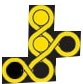
\includegraphics[width=0.75\textwidth]{figs/yellow2.jpg}
\caption{Initial state of yellow2}
  \label{fig:2Dyellow2}
\end{subfigure}
\begin{subfigure}[b]{.24\textwidth}
\centering
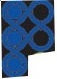
\includegraphics[width =0.5\textwidth]{figs/blue1.jpg}
\caption{Initial state of blue1}
  \label{fig:2Dblue1}
\end{subfigure}
\begin{subfigure}[b]{.24\textwidth}
\centering

\includegraphics[width=\textwidth]{figs/blue2.jpg}
\caption{Initial state of blue2}
  \label{fig:2Dblue2}
\end{subfigure}
\begin{subfigure}[b]{.24\textwidth}
\centering

\includegraphics[width=0.75\textwidth]{figs/green1.jpg}
\caption{Initial state of green1}
  \label{fig:2Dgreen1}
\end{subfigure}
\begin{subfigure}[b]{.24\textwidth}
\centering

\includegraphics[width =0.5\textwidth]{figs/green2.jpg}
\caption{Initial state of green2}
  \label{fig:2Dgreen2}
\end{subfigure}
\begin{subfigure}[b]{.24\textwidth}
\centering

\includegraphics[width =\textwidth]{figs/red1.jpg}
\caption{Initial state of red1}
  \label{fig:2Dred1}
\end{subfigure}
\begin{subfigure}[b]{.24\textwidth}
\centering

\includegraphics[width=0.75\textwidth]{figs/red2.jpg}
\caption{Initial state of red2}
  \label{fig:2Dred2}
\end{subfigure}
\caption{Initial state of each piece}
  \label{fig:allinit}
\end{figure}
For this model, there are some rules. Firstly, all the variables are corresponding to the specific units. As an example, for piece yellow2, Figure~\ref{fig:namerules} shows that the $V_{y21}$ is used to represent the left and bottom unit. For other variables, we name them as $V_{y22}$, $V_{y23}$, $V_{y24}$ and $V_{y25}$, which follows the order from left to right and bottom-up. In addition, there are 7 pegs. Therefore, the variables can be represented as \VUnits and \VPegs,
\begin{equation}
\begin{aligned}
\VUnits=\{&V_{y11},V_{y12},V_{y13},\\&V_{y21},V_{y22},V_{y23},V_{y24},V_{y25},\\&V_{b11},V_{b12},V_{b13},V_{b14},
V_{b15},\\&V_{b21},V_{b22},V_{b23},V_{b24},\\&V_{g11},V_{g12},V_{g13},V_{g14},\\&V_{g21},V_{g22},V_{g23},\\&V_{r11},
V_{r12},V_{r13},V_{r14},\\&V_{r21},V_{r22},V_{r23},V_{r24}\},\\
\\\VPegs = \{&V_{py1}, V_{py2}, V_{pb1}, V_{pb2}, V_{pg1}, V_{pg2}, V_{pr}\},\\
\\V = &\VUnits \cup \VPegs.
\end{aligned}
\end{equation}
\begin{figure}[htbp]
    \centering
    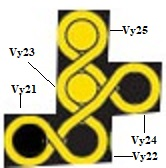
\includegraphics[width=0.3\textwidth]{figs/example.jpg}
    \caption{Name rules for yellow2}
    \label{fig:namerules}
\end{figure}
\subsection{Domains}
\begin{figure}[htbp]
\centering
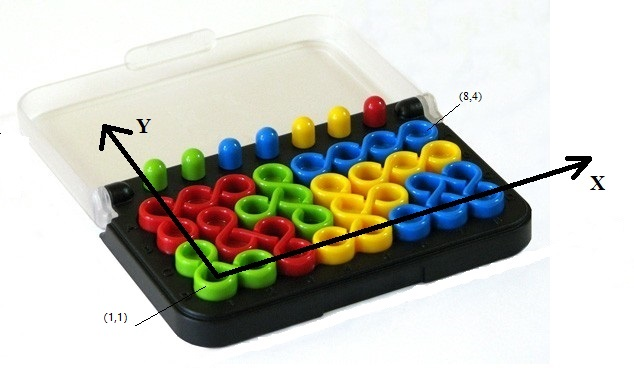
\includegraphics[width=0.8\textwidth]{figs/IQtwistboard.jpg}
\caption{The coordinate system for IQ twist}
    \label{fig:coordinate}
\end{figure}
For the board, Figure~\ref{fig:coordinate} shows that the 2D coordinate system is used to represent the positions. In our model, all positions are represented as tuples and the elements in the tuples are int. In addition, each tuple contains 2 int. The left and bottom position as $(1,1)$ and the right and top as $(8,4)$. So, all placements will be between them. Considering a position $(x_{0},y_{0})$, we get
\begin{equation}
\begin{aligned}
&0<x_{0} \leq 8,\\
&0<y_{0} \leq 4.
\end{aligned}
\end{equation}
The placements for each unit of pieces must on the board, therefore, we get
\begin{equation}
\forall  v \in \VUnits \hspace{1ex},\hspace{1ex} D(v)=\{(i,j) \in \mathbb{Z} \times \mathbb{Z}	\mid  0<i \leq 8 \hspace{1ex} , \hspace{1ex} 0<j \leq 4\}.\\
\end{equation}
The pegs are special because they can be put in any places on the board or not on the board. So, the domain of pegs is
\begin{equation}
\forall  v \in \VPegs \hspace{1ex},\hspace{1ex} D(v)=\{(0,0)\} \hspace{1ex} \cup \hspace{1ex}\{(i,j) \in \mathbb{Z} \times \mathbb{Z}\mid  0<i \leq 8 \hspace{1ex} , \hspace{1ex} 0<j \leq 4\}.
\end{equation}
\subsection{2D Rotation Matrix}
\label{section:2Drotationmatrix}
To clarify how to obtain all configurations for each piece. I'd like to introduce 2D rotation matrix. In Figure~\ref{fig:explanation2D}, the unit which is corresponding to the first variable ($V_{y21}$) will be considered as a point $(x_{0},y_{0})$. Therefore, the $V_{y21}$, $V_{y22}$, $V_{y23}$, $V_{y24}$ and $V_{y25}$ are respectively represented as $(x_{0},y_{0})$, $(x_{0}+1,y_{0})$, $(x_{0}+1,y_{0}+1)$, $(x_{0}+2,y_{0}+1)$ and $(x_{0}+1,y_{0}+2)$, which indicate that all other variables are connection with the first variables.
\begin{figure}[htbp]
\centering
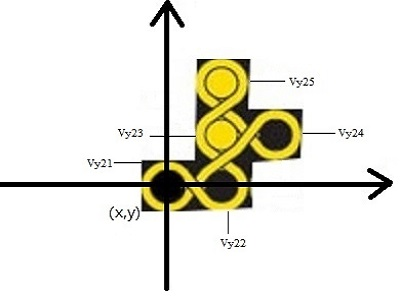
\includegraphics[width=0.5\textwidth]{figs/explanation2D.jpg}
\caption{The explanation of 2D rotation}
    \label{fig:explanation2D}
\end{figure}
Therefore, all other placements can be obtained from the initial state of the piece by rotations around the unit of $V_{y21}$.\\
Tobias and Krantz \cite{r9} mention that 2D rotation by an angle $\theta$ around the origin of coordinate can be described as a matrix
\begin{equation}
R(\theta)=\begin{bmatrix}
\cos\theta & -\sin\theta\\
\sin\theta & \cos\theta\\
\end{bmatrix}.
\end{equation}
If the initial position is (x,y), we can get the position after the rotation by
\begin{equation}
\label{equation:rotation}
\begin{bmatrix}
x'\\
y'\\
\end{bmatrix}
=\begin{bmatrix}
\cos\theta & -\sin\theta\\
\sin\theta & \cos\theta\\
\end{bmatrix}
\begin{bmatrix}
x\\
y\\
\end{bmatrix},
\end{equation}
which implies that 
\begin{equation}
\label{equation:formula1}
\begin{aligned}
&x'=x\cos\theta-y\sin\theta,\\
&y'=x\sin\theta+y\cos\theta.
\end{aligned}
\end{equation}
Therefore, if we assign 0, 90, 180 and 270 degrees to $\theta$, we get four configurations:
\begin{itemize}
  \item $x'=x\cos0^{\circ} - y\sin0^{\circ}\hspace{20pt},y'=x\sin0^{\circ} + y\cos0^{\circ}\hspace{24pt}\implies x'=x\hspace{10pt}, y'=y$
  \item $x'=x\cos90^{\circ} - y\sin90^{\circ}\hspace{10pt},y'=x\sin90^{\circ} + y\cos90^{\circ}\hspace{12pt}\implies x'=-y, y'=x$
  \item $x'=x\cos180^{\circ} - y\sin180^{\circ}, y'=x\sin180^{\circ} + y\cos180^{\circ} \implies x'=-x, y'=-y$
  \item $x'=x\cos270^{\circ} - y\sin270^{\circ}, y'=x\sin270^{\circ} + y\cos270^{\circ} \implies x'=y\hspace{10pt},y'=-x$
  \label{rotation4}
\end{itemize}
In IQ twist, there exists a mirroring operation which corresponds to flpping a piece, if a unit of piece flip over around the y-axis, we get  (-x,y) from (x,y). Similarly, all the four configurations flip over around the y-axis. We get four more configurations: 
\begin{itemize}
  \item  $x'=x\hspace{10pt}, y'=y\hspace{10pt}$    flip over around the y-axis $\implies x''=-x\hspace{8pt},y''=y$
  \item  $x'=-y, y'=x\hspace{10pt}$                flip over around the y-axis $\implies x''=y,y''=x$
  \item  $x'=-x, y'=-y$               flip over around the y-axis $\implies x''=x, y''=-y$
  \item  $x'=y\hspace{10pt},y'=-x$    flip over around the y-axis $\implies x''=-y\hspace{8pt}, y''=-x$
  \label{mirrorrotate4}
\end{itemize}
Therefore, there should be a total of eight configurations for each unit of pieces. Similarly, in Figure~\ref{fig:explanation2D}, if we assign $(0,0)$ to $(x_{0},y_{0})$, the process of rotation for each other unit of the piece can be represented by equation~\ref{equation:rotation}. Accordingly, we get
\begin{itemize}
 \item $V_{y21}=(0,0)$, $V_{y22}=(1,0)$, $V_{y23}=(1,1)$, $V_{y24}=(2,1)$, $V_{y25}=(1,2)$ or
 \item $V_{y21}=(0,0)$, $V_{y22}=(0,1)$, $V_{y23}=(-1,1)$, $V_{y24}=(-1,2)$, $V_{y25}=(-2,1)$ or
 \item $V_{y21}=(0,0)$, $V_{y22}=(-1,0)$, $V_{y23}=(-1,-1)$, $V_{y24}=(-2,-1)$, $V_{y25}=(-1,-2)$ or
 \item $V_{y21}=(0,0)$, $V_{y22}=(0,-1)$, $V_{y23}=(1,-1)$, $V_{y24}=(1,-2)$, $V_{y25}=(2,-1)$ or
 \item $V_{y21}=(0,0)$, $V_{y22}=(-1,0)$, $V_{y23}=(-1,1)$, $V_{y24}=(-2,1)$, $V_{y25}=(-1,2)$ or
 \item $V_{y21}=(0,0)$, $V_{y22}=(0,1)$, $V_{y23}=(1,1)$, $V_{y24}=(1,2)$, $V_{y25}=(2,1)$ or
 \item $V_{y21}=(0,0)$, $V_{y22}=(1,0)$, $V_{y23}=(1,-1)$, $V_{y24}=(2,-1)$, $V_{y25}=(1,-2)$ or
 \item $V_{y21}=(0,0)$, $V_{y22}=(-1,0)$, $V_{y23}=(-1,-1)$, $V_{y24}=(-2,-1)$, $V_{y25}=(-1,-2)$.
\end{itemize}
In our case, the piece can be moved only if all units of piece on the board. So both the $x_{0}$ and $y_{0}$ can be variables, we get
\begin{itemize}
 \item $V_{y21}=(x_{0},y_{0})$, $V_{y22}=(x_{0}+1,y_{0})$, $V_{y23}=(x_{0}+1,y_{0}+1)$, $V_{y24}=(x_{0}+2,y_{0}+1)$, $V_{y25}=(x_{0}+1,y_{0}+2)$ or
 \item $V_{y21}=(x_{0},y_{0})$, $V_{y22}=(x_{0},y_{0}+1)$, $V_{y23}=(x_{0}-1,y_{0}+1)$, $V_{y24}=(x_{0}-1,y_{0}+2)$, $V_{y25}=(x_{0}-2,y_{0}+1)$ or
 \item $V_{y21}=(x_{0},y_{0})$, $V_{y22}=(x_{0}-1,y_{0})$, $V_{y23}=(x_{0}-1,y_{0}-1)$, $V_{y24}=(x_{0}-2,y_{0}-1)$, $V_{y25}=(x_{0}-1,y_{0}-2)$ or
 \item $V_{y21}=(x_{0},y_{0})$, $V_{y22}=(x_{0},y_{0}-1)$, $V_{y23}=(x_{0}+1,y_{0}-1)$, $V_{y24}=(x_{0}+1,y_{0}-2)$, $V_{y25}=(x_{0}+2,y_{0}-1)$ or
 \item $V_{y21}=(x_{0},y_{0})$, $V_{y22}=(x_{0}-1,y_{0})$, $V_{y23}=(x_{0}-1,y_{0}+1)$, $V_{y24}=(x_{0}-2,y_{0}+1)$, $V_{y25}=(x_{0}-1,y_{0}+2)$ or
 \item $V_{y21}=(x_{0},y_{0})$, $V_{y22}=(x_{0},y_{0}+1)$, $V_{y23}=(x_{0}+1,y_{0}+1)$, $V_{y24}=(x_{0}+1,y_{0}+2)$, $V_{y25}=(x_{0}+2,y_{0}+1)$ or
 \item $V_{y21}=(x_{0},y_{0})$, $V_{y22}=(x_{0}+1,y_{0})$, $V_{y23}=(x_{0}+1,y_{0}-1)$, $V_{y24}=(x_{0}+2,y_{0}-1)$, $V_{y25}=(x_{0}+1,y_{0}-2)$ or
 \item $V_{y21}=(x_{0},y_{0})$, $V_{y22}=(x_{0}-1,y_{0})$, $V_{y23}=(x_{0}-1,y_{0}-1)$, $V_{y24}=(x_{0}-2,y_{0}-1)$, $V_{y25}=(x_{0}-1,y_{0}-2)$.
\end{itemize}
\subsection{Constrains}
Firstly, there should be no 2 different unit variables contain the same value
\begin{equation}
\begin{aligned}
&\forall V_{m},V_{n} \in \VUnits,V_{m} \neq V_{n},\\
&\Constraints{m}{n}=\{((x_{1},y_{1}),(x_{2},y_{2}))\in \Domain{m} \times \Domain{n}\mid x_{1} \neq x_{2}   \hspace{1ex} or \hspace{1ex}  y_{1} \neq y_{2}\}.
\end{aligned}
\end{equation}
Similarly, there should be no 2 different reg variables contain the same value except both of them are not on the board
\begin{equation}
\begin{aligned}
&\forall V_{m},V_{n}\in \VPegs, V_{m} \neq V_{n},\\
&\Constraints{m}{n}=\{((x_{1},y_{1}),(x_{2},y_{2}))\in \Domain{m}\times \Domain{n}\mid x_{1} \neq x_{2}   \hspace{1ex} or \hspace{1ex}  y_{1} \neq y_{2}\}\hspace{1pt}\cup \\
&\{((0,0),(0,0))\}.
\end{aligned}
\end{equation}
As is mentioned in Chapter~\ref{section:2Drotationmatrix}, there should be eight configurations for general pieces. Figure~\ref{fig:Exampleof8} shows the eight configurations for yellow2. Hence,
\begin{figure}[htbp]
\centering
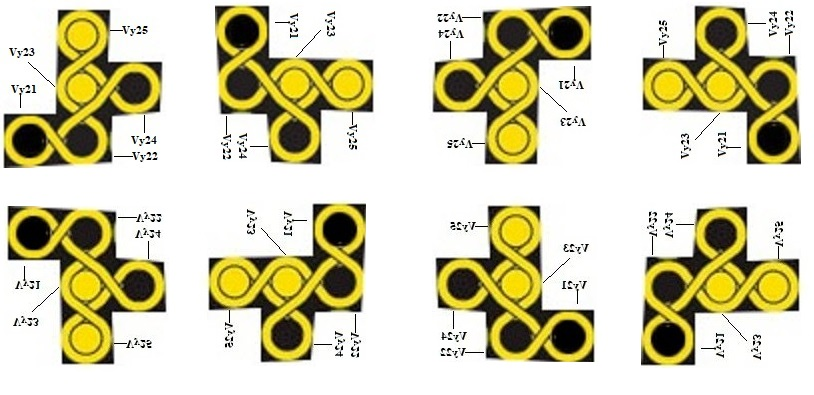
\includegraphics[width =\textwidth]{figs/domainexplain.jpg}
    \caption{Example of 8 configurations}
    \label{fig:Exampleof8}
\end{figure}
\begin{equation}
\begin{aligned}
\Cons{y21}{y22}{y23}{y24}{y25}=\{&((x_{1},y_{1}),(x_{2},y_{2}),(x_{3},y_{3}),(x_{4},y_{4}),(x_{5},y_{5}))\in \\
&\Domain {y21} \times \Domain{y22}\times \Domain{y23}\times \Domain{y24}\times \Domain{y25} \mid\\
&(x_{2} = x_{1} + 1,\hspace{1ex}y_{2} = y_{1},\hspace{1ex}x_{3} = x_{1}+1,\hspace{1ex}y_{3} = y_{1}+1,
\\&x_{4} = x_{1}+2,\hspace{1ex}y_{4} = y_{1}+1,\hspace{1ex}x_{5} = x_{1}+1,\hspace{1ex}y_{5} = y_{1}+2)\hspace{1ex} or \\
&(x_{2} = x_{1} ,\hspace{1ex}y_{2} = y_{1}+1,\hspace{1ex}x_{3} = x_{1}-1,\hspace{1ex}y_{3} = y_{1}+1,
\\&x_{4} = x_{1}-1,\hspace{1ex}y_{4} = y_{1}+2,\hspace{1ex}x_{5} = x_{1}-2,\hspace{1ex}y_{5} = y_{1}+1)\hspace{1ex} or \\
&(x_{2} = x_{1}-1 ,\hspace{1ex}y_{2} = y_{1},\hspace{1ex}x_{3} = x_{1}-1,\hspace{1ex}y_{3} = y_{1}-1,
\\&x_{4} = x_{1}-2,\hspace{1ex}y_{4} = y_{1}-1,\hspace{1ex}x_{5} = x_{1}-1,\hspace{1ex}y_{5} = y_{1}-2)\hspace{1ex} or \\
&(x_{2} = x_{1} ,\hspace{1ex}y_{2} = y_{1}-1,\hspace{1ex}x_{3} = x_{1}+1,\hspace{1ex}y_{3} = y_{1}-1,
\\&x_{4} = x_{1}+1,\hspace{1ex}y_{4} = y_{1}-2,\hspace{1ex}x_{5} = x_{1}+2,\hspace{1ex}y_{5} = y_{1}-1)\hspace{1ex} or \\
&(x_{2} = x_{1}-1 ,\hspace{1ex}y_{2} = y_{1},\hspace{1ex}x_{3} = x_{1}-1,\hspace{1ex}y_{3} = y_{1}+1,
\\&x_{4} = x_{1}-2,\hspace{1ex}y_{4} = y_{1}+1,\hspace{1ex}x_{5} = x_{1}-1,\hspace{1ex}y_{5} = y_{1}+2)\hspace{1ex} or \\
&(x_{2} = x_{1} ,\hspace{1ex}y_{2} = y_{1}-1,\hspace{1ex}x_{3} = x_{1}-1,\hspace{1ex}y_{3} = y_{1}-1,
\\&x_{4} = x_{1}-1,\hspace{1ex}y_{4} = y_{1}-2,\hspace{1ex}x_{5} = x_{1}-2,\hspace{1ex}y_{5} = y_{1}-1)\hspace{1ex} or \\
&(x_{2} = x_{1}+1 ,\hspace{1ex}y_{2} = y_{1},\hspace{1ex}x_{3} = x_{1}+1,\hspace{1ex}y_{3} = y_{1}-1,
\\&x_{4} = x_{1}+2,\hspace{1ex}y_{4} = y_{1}-1,\hspace{1ex}x_{5} = x_{1}+1,\hspace{1ex}y_{5} = y_{1}-2)\hspace{1ex} or \\
&(x_{2} = x_{1} ,\hspace{1ex}y_{2} = y_{1}+1,\hspace{1ex}x_{3} = x_{1}+1,\hspace{1ex}y_{3} = y_{1}+1,
\\&x_{4} = x_{1}+1,\hspace{1ex}y_{4} = y_{1}+2,\hspace{1ex}x_{5} = x_{1}+2,\hspace{1ex}y_{5} = y_{1}+1)\hspace{3ex}\}.
\end{aligned}
\end{equation}
Similarly, every piece can get the similar constraints (Appendix~\ref{appendix:2Dpieces}). Furthermore, for the pegs, unless they are not on the board, there must be a hollow unit of pieces which contains the same color with the pegs to match them. As an instance, for yellow peg1, there are 4 hollow units of yellow pieces. Therefore, we can obtain
\begin{equation}
\begin{aligned}  
\Constraint{py1} = &\{((x_{1},y_{1}),(x_{2},y_{2}))\in \Domain{py1} \times \Domain{y11}\mid x_{2} = x_{1} \hspace{1ex} , \hspace{1ex}  y_{2} = y_{1}\}\hspace{1ex} \cup  
\\&\{((x_{1},y_{1}),(x_{2},y_{2}))\in \Domain{py1} \times \Domain{y21}\mid x_{2} = x_{1} \hspace{1ex} , \hspace{1ex}  y_{2} = y_{1}\}\hspace{1ex} \cup 
\\&\{ ((x_{1},y_{1}),(x_{2},y_{2}))\in \Domain{py1} \times \Domain{y22}\mid x_{2} = x_{1} \hspace{1ex} , \hspace{1ex}  y_{2} = y_{1}\}\hspace{1ex}\cup 
\\& \{((x_{1},y_{1}),(x_{2},y_{2}))\in \Domain{py1} \times \Domain{y24}\mid x_{2} = x_{1} \hspace{1ex} , \hspace{1ex}  y_{2} = y_{1}\} \hspace{1ex}\cup
\\& \{(0,0)\}.
\end{aligned}
\end{equation}
Accordingly, every peg can get the similar constraints (Appendix~\ref{appendix:2Dpegs}).
\section{ZIG ZAG Puzzler}
Zig Zag Puzzler is a 3D puzzle game with 2 playing modes. Both games aim to place all pieces to full fill the game boards. In addition, for both of them, there are some pieces placed in advance to adjust the difficulty (Figure~\ref{fig:ZIG_ZAG_Puzzler_playing_modes}). Generally, the fewer pieces are placed in advance, the more difficult.
\begin{figure}[htbp]
    \centering
    \begin{subfigure}[b]{0.4\textwidth}
    
\includegraphics[width=\textwidth]{figs/zig_zag_mode1.jpg}
    \caption{One example of ZIG ZAG Puzzler mode1}
    \end{subfigure}
    \begin{subfigure}[b]{0.4\textwidth}
    
\includegraphics[width=\textwidth]{figs/zig_zag_mode2.jpg}
    \caption{One example of ZIG ZAG Puzzler mode2}
    \end{subfigure}
    \caption{ZIG ZAG Puzzler examples}
    \label{fig:ZIG_ZAG_Puzzler_playing_modes}
\end{figure}
\\In this part, the designs of CSP models for ZIG ZAG Puzzler will be discussed. For the ZIG ZAG Puzzler, there are 2 playing modes, which uses the same pieces but different boards. On the condition of the two coordinates based on the same system which means both of them adopt right-hand system or left-hand system, both of them can adopt the same variables and the same constraints but different domains. In our case, we adopt right-hand system. 
\subsection{Variables}
Firstly, the initial state of each piece is defined in Figure~\ref{fig:all3Dinit}.
\label{section:3Dgame}
\begin{figure}[htbp]
\centering
\begin{subfigure}[b]{0.25\textwidth}
\centering
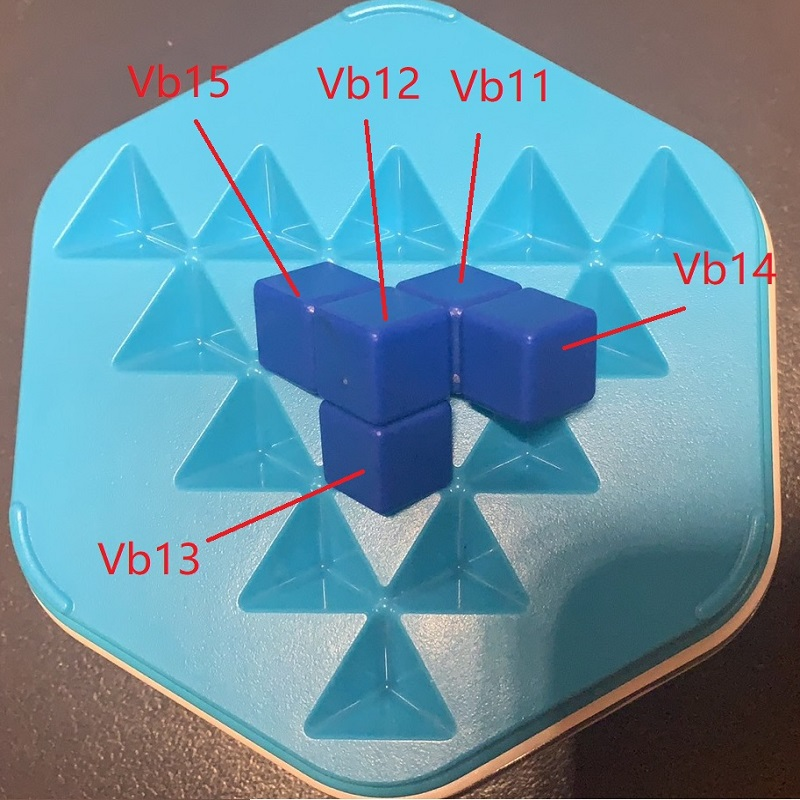
\includegraphics[width=\textwidth]{figs/3Dblue1.jpg}
\caption{The variable explanation of blue1}
  \label{fig:3Dblue1}
\end{subfigure}
\begin{subfigure}[b]{0.25\textwidth}
\centering
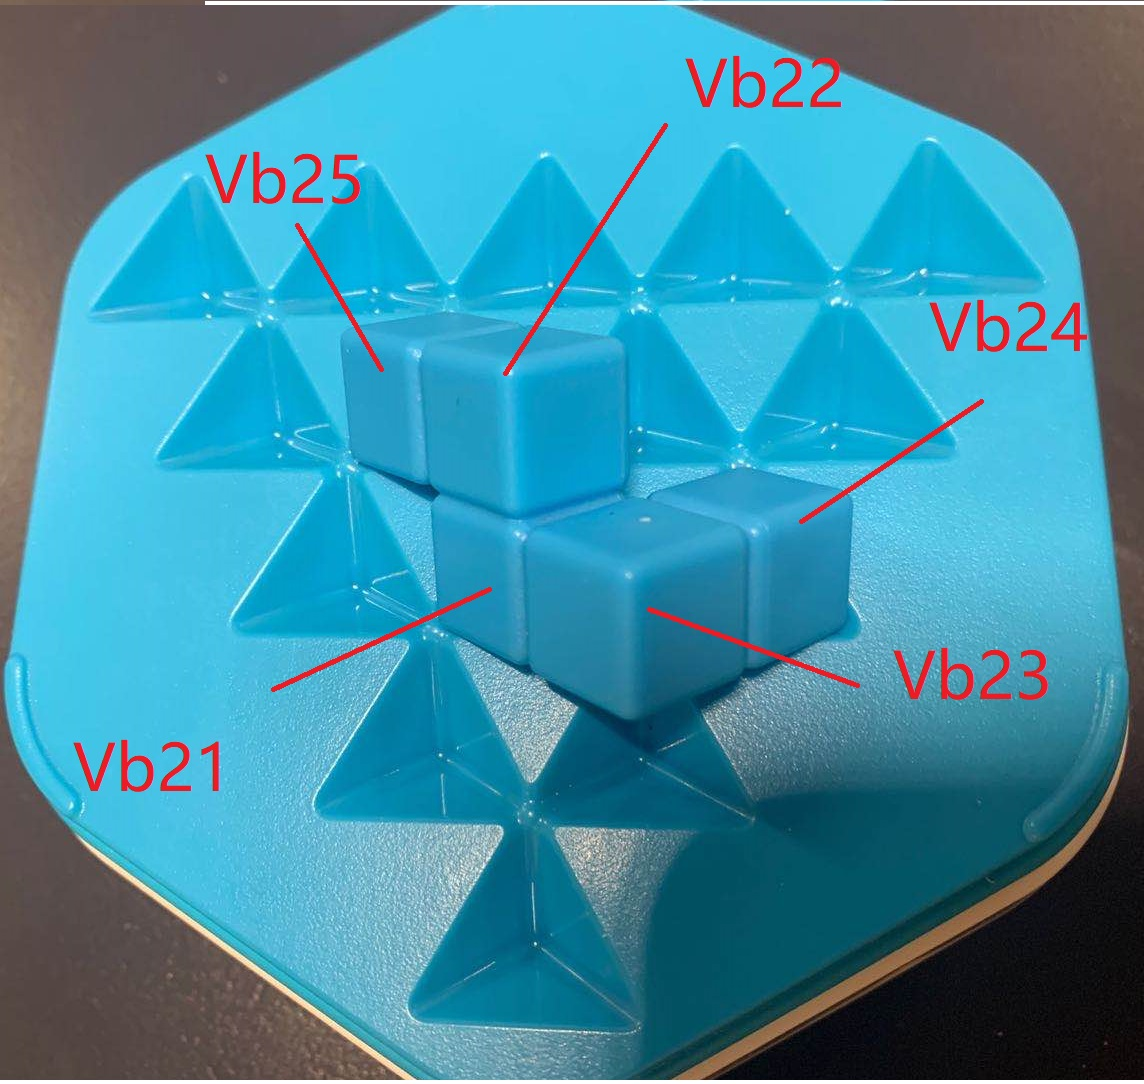
\includegraphics[width=\textwidth]{figs/3Dblue2.jpg}
\caption{The variable explanation of blue2}
  \label{fig:3Dblue2}
\end{subfigure}
\begin{subfigure}[b]{0.25\textwidth}
\centering
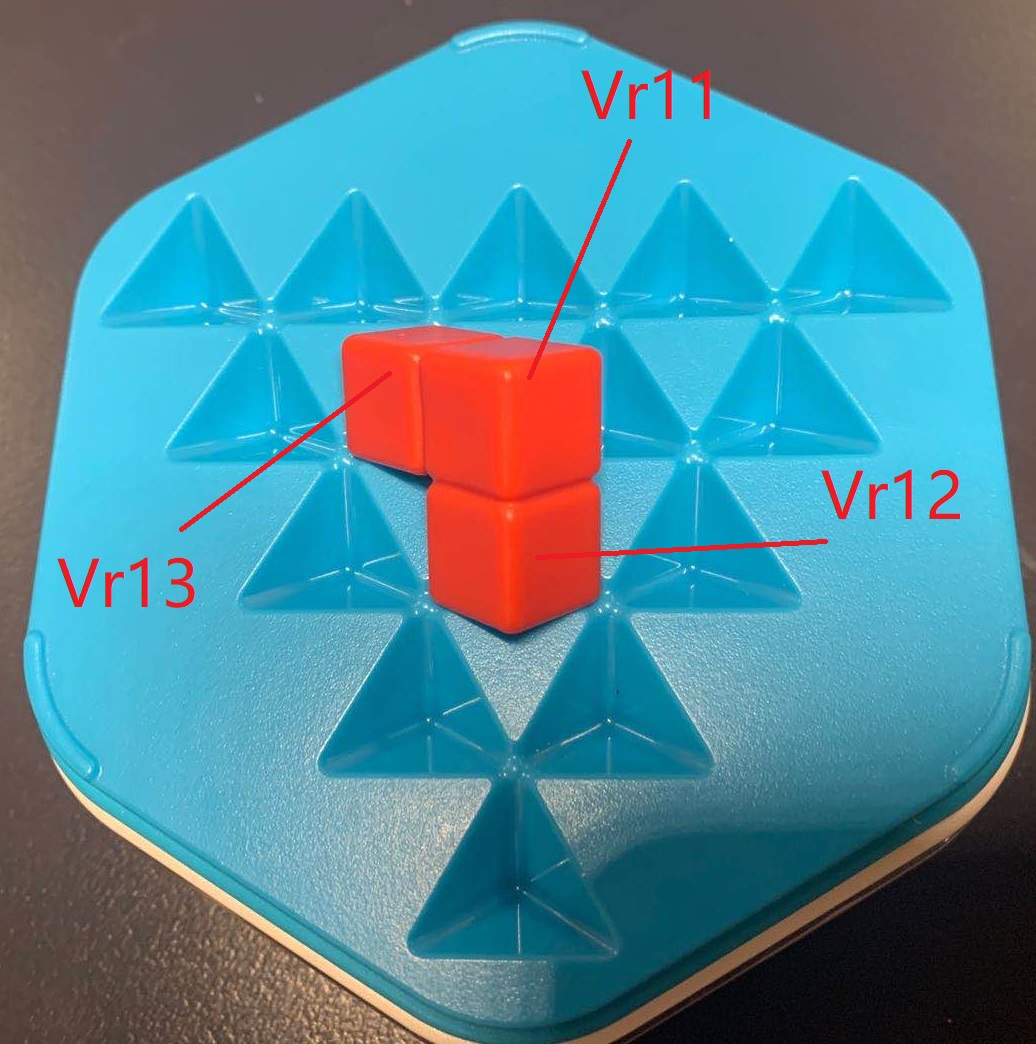
\includegraphics[width=\textwidth]{figs/3Dred1.jpg}
\caption{The variable explanation of red1}
  \label{fig:3Dred1}
\end{subfigure}
\begin{subfigure}[b]{0.25\textwidth}
\centering
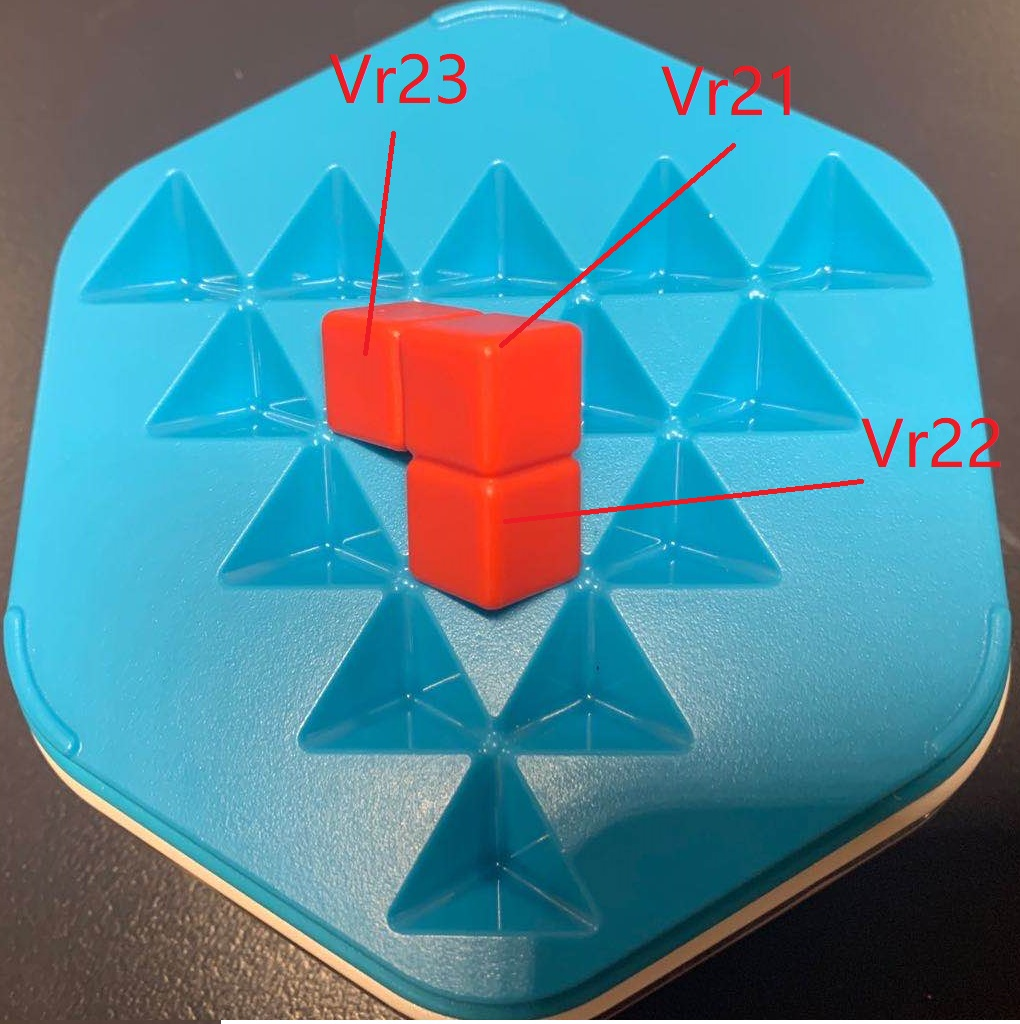
\includegraphics[width=\textwidth]{figs/3Dred2.jpg}
\caption{The variable explanation of red2}
  \label{fig:3Dred2}
\end{subfigure}
\begin{subfigure}[b]{0.25\textwidth}
\centering
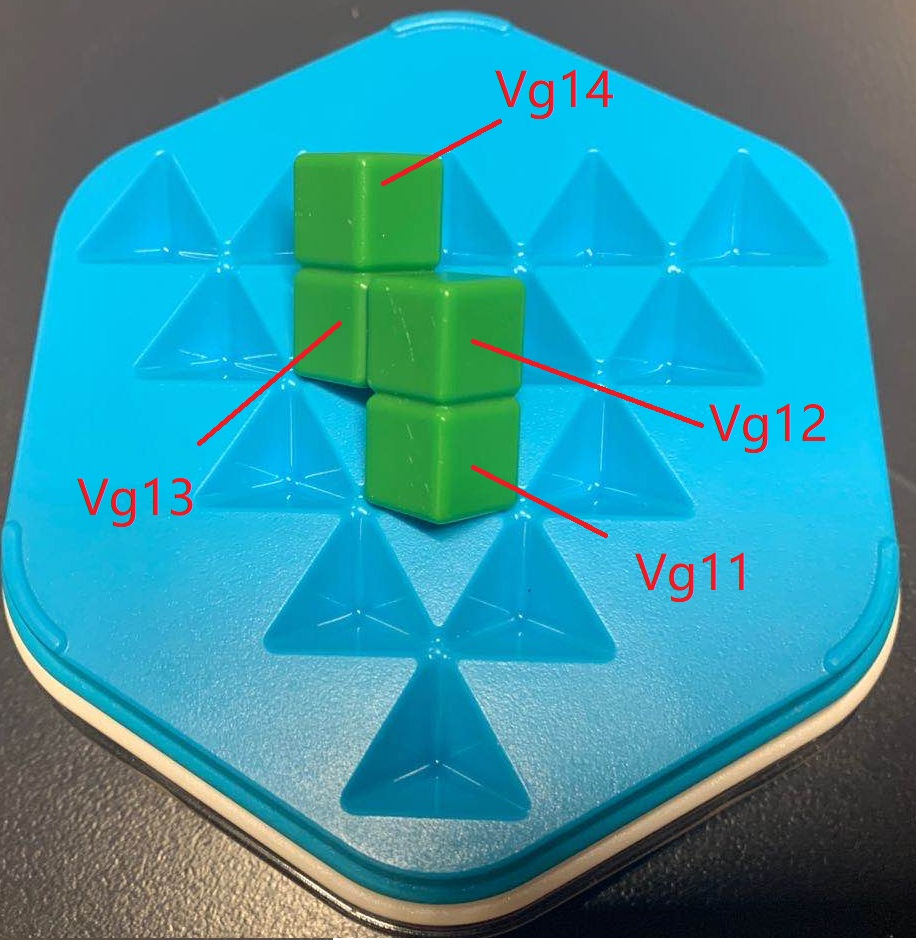
\includegraphics[width=\textwidth]{figs/3Dgreen1.jpg}
\caption{The variable explanation of green1}
  \label{fig:3Dgreen1}
\end{subfigure}
\begin{subfigure}[b]{0.25\textwidth}
\centering
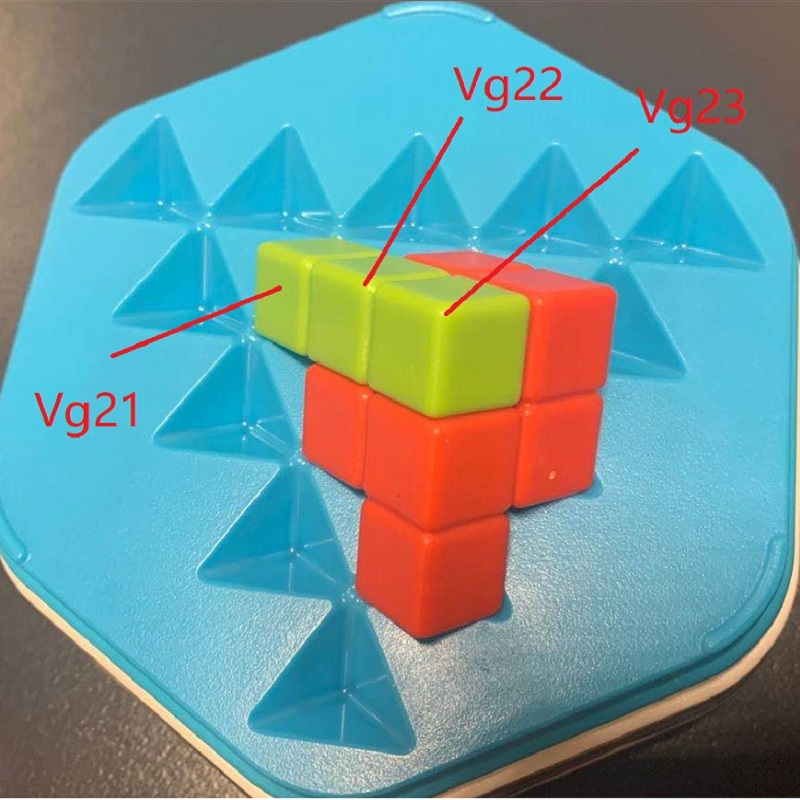
\includegraphics[width=\textwidth]{figs/3Dgreen2.jpg}
\caption{The variable explanation of green2}
  \label{fig:3Dgreen2}
\end{subfigure}
\begin{subfigure}[b]{0.25\textwidth}
\centering
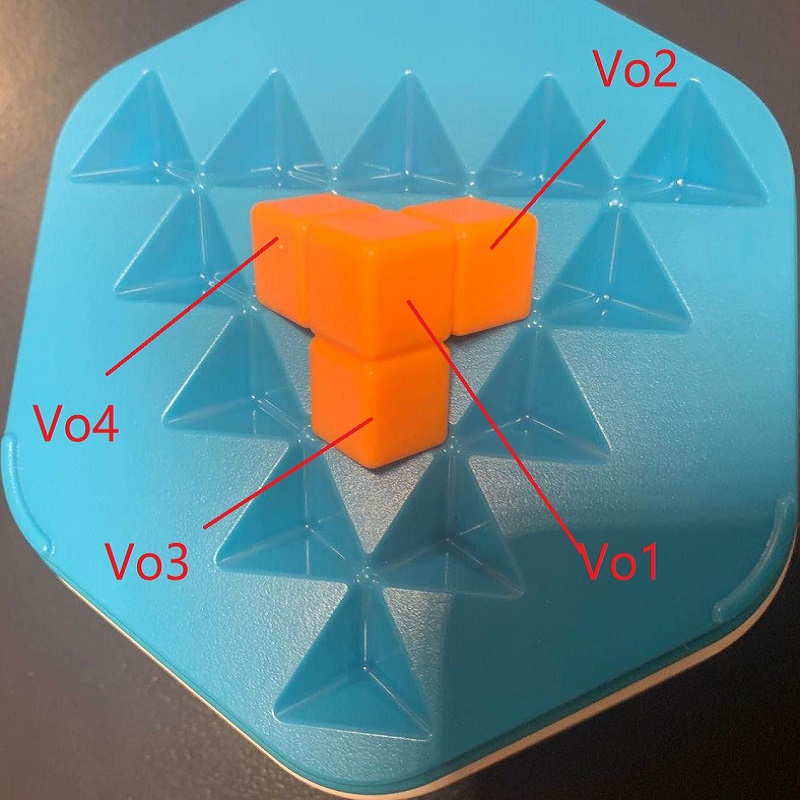
\includegraphics[width=\textwidth]{figs/3Dorange.jpg}
\caption{The variable explanation of orange}
  \label{fig:3Dorange}
\end{subfigure}
\begin{subfigure}[b]{0.25\textwidth}
\centering
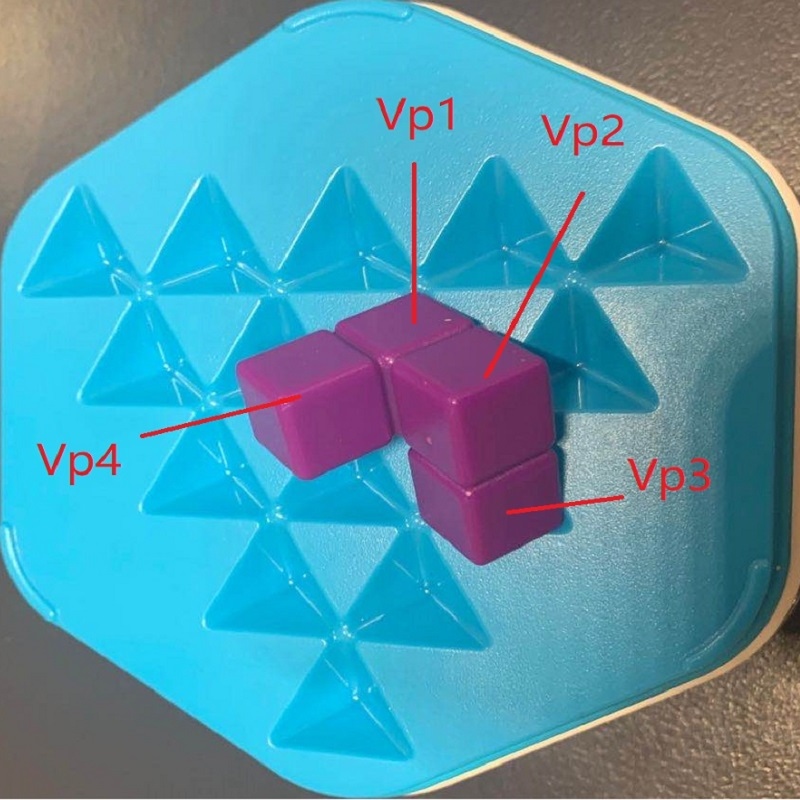
\includegraphics[width=\textwidth]{figs/3Dpurple.jpg}
\caption{The variable explanation of purple}
  \label{fig:3Dpurple}
\end{subfigure}
\begin{subfigure}[b]{0.25\textwidth}
\centering
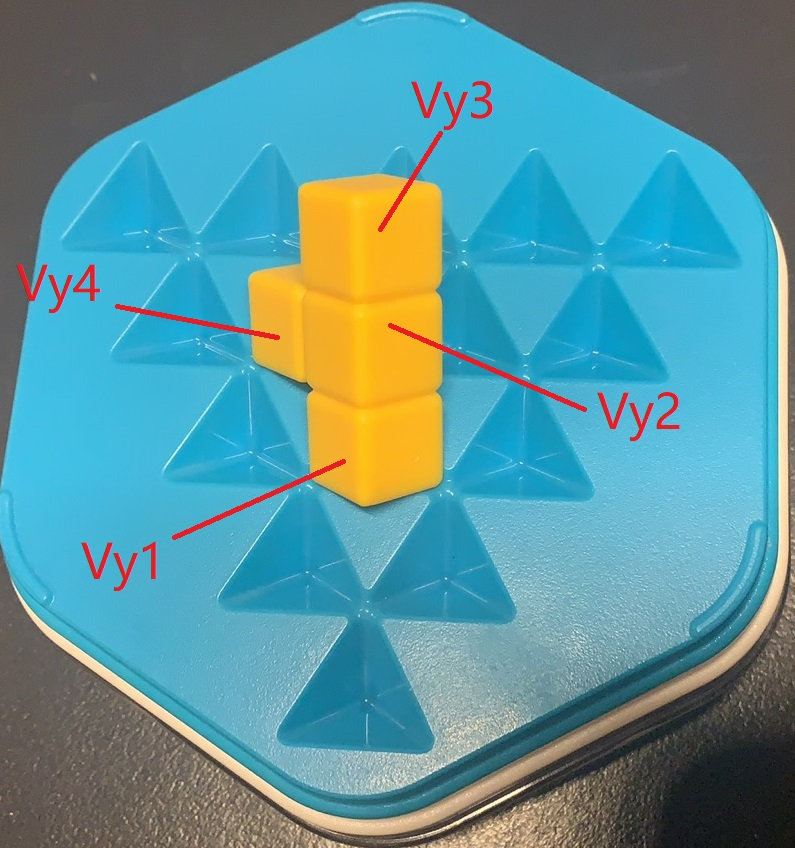
\includegraphics[width=\textwidth]{figs/3Dyellow.jpg}
\caption{The variable explanation of yellow}
  \label{fig:3Dyellow}
\end{subfigure}
\caption{Initial state of each piece}
  \label{fig:all3Dinit}
\end{figure}
It shows all the variables are corresponding to the specific units. Therefore, the variables can be defined as
\begin{equation}
\begin{aligned}
\VUnits=\{&V_{y1},V_{y2},V_{y3},V_{y4},\\&V_{b11},V_{b12},V_{b13},V_{b14},
V_{b15},\\&V_{b21},V_{b22},V_{b23},V_{b24},V_{b25},\\&V_{g11},V_{g12},V_{g13},V_{g14},\\&V_{g21},V_{g22},V_{g23},\\&V_{r11},
V_{r12},V_{r13},\\&V_{r21},V_{r22},V_{r23},\\&V_{o1},V_{o2},V_{o3},V_{o4},\\&V_{p1},V_{p2},V_{p3},V_{p4}\}.
\end{aligned}
\end{equation}
\subsection{Domains for Playing Mode 1 and 2}
\label{sec:3Ddomains}
Figure~\ref{fig:board1} and Figure~\ref{fig:board2} show how to create the coordinates for both modes to represent the positions of the boards. For both modes, similar to IQ twist, the positions are represented as tuples and the elements in tuples are int. But each tuple will contain 3 int. The unit of piece which is located in the origin of coordinate can be represented as $(1,1,1)$. So Considering one position $(x_{0},y_{0},z_{0})$.
\begin{figure}[htbp]
\centering
\begin{subfigure}[b]{.4\textwidth}
\centering
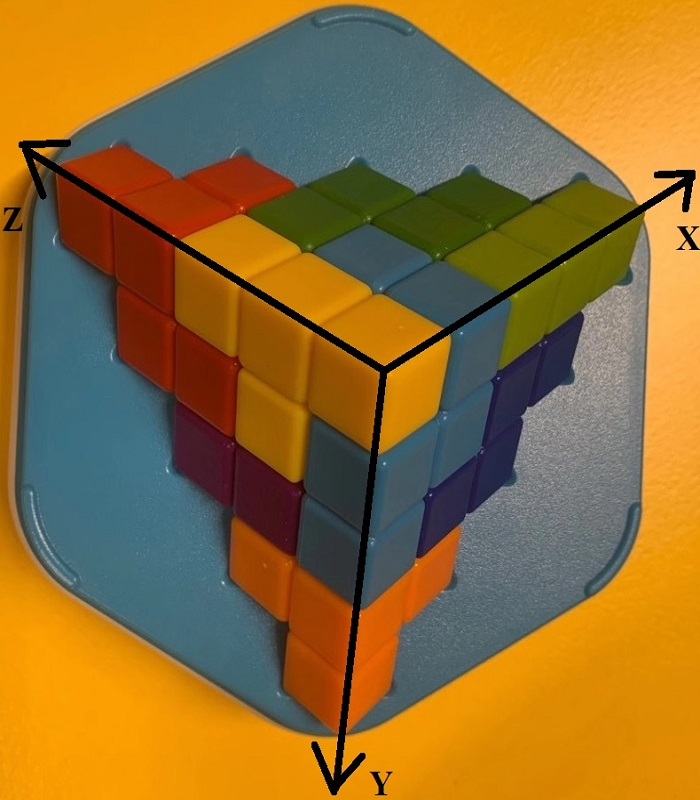
\includegraphics[width=\textwidth]{figs/ZIGZAGmodel1board.jpg}
\caption{}
\label{figure:mode1A}
\end{subfigure}
\begin{subfigure}[b]{.4\textwidth}
\centering
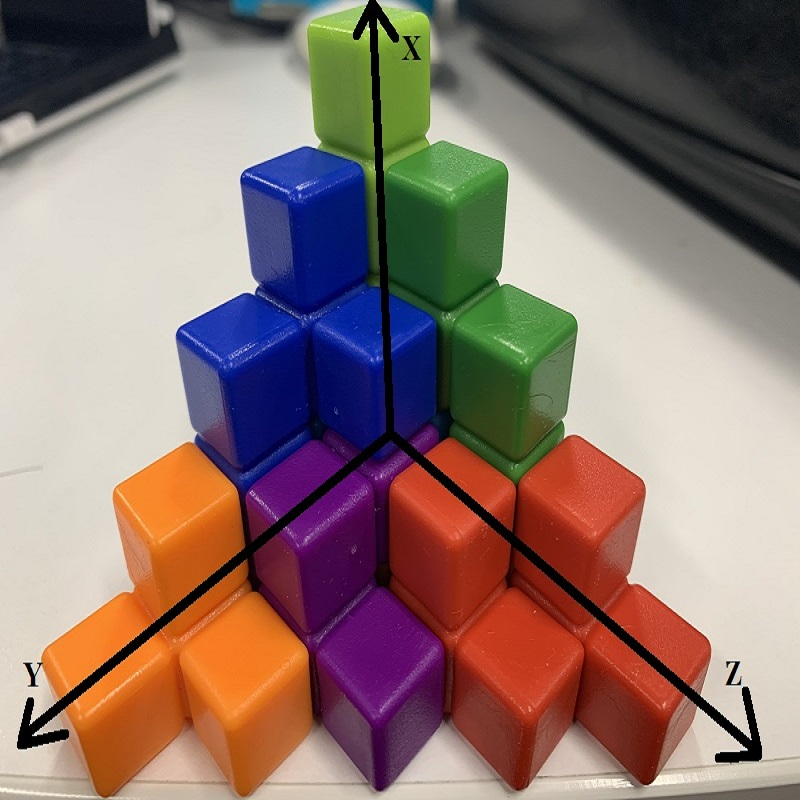
\includegraphics[width=\textwidth]{figs/3Dboard1.jpg}
\caption{}
\label{figure:mode1B}
\end{subfigure}
\caption{The board of ZIA ZAG Puzzler mode1}
  \label{fig:board1}
\end{figure}
\\For playing mode1, as is shown in Figure~\ref{fig:board1}, the maximum number for each axis is 5, hence,
\begin{equation}
\begin{aligned}
&0<x_{0}\leq5,\\
&0<y_{0}\leq5,\\
&0<z_{0}\leq5.
\end{aligned}
\end{equation}
If it is located in one of the 3 plane. Such as xy-plane $(x_{0},y_{0},1)$, it will satisfy
\begin{equation}
x_{0}+y_{0}\leq6.
\end{equation}
Accordingly, it will satisfy 
\begin{equation}
x_{0}+z_{0}\leq6
\end{equation}
in xz-plane and 
\begin{equation}
y_{0}+z_{0}\leq6
\end{equation}
in yz-plane. In addition, Figure~\ref{figure:mode1B} shows that all the units that are not in the 3 planes are close to one of the three planes, which means it's a unit of distance to one of the three plane. So we get
\begin{equation}
x_{0}+y_{0}+z_{0}\leq7.
\end{equation}
Because what we discussed above has included all positions, the domain of playing mode1 is
\begin{equation}
\begin{aligned}
&\forall \hspace{1ex} v \in \VUnits,\\
&D(v)=\{(x,y,z) \in \mathbb{Z} \times \mathbb{Z}	\times \mathbb{Z} \mid  0<x \leq 5, \hspace{1ex} 0<y \leq 5,\hspace{1ex} 0<z \leq 5,\\ &x+y\leq 6,\hspace{1ex} y+z\leq 6,\hspace{1ex}x+z\leq 6,\hspace{1ex}x+y+z\leq 7\}.
\end{aligned}
\end{equation}
\begin{figure}[htbp]
\centering
\begin{subfigure}[b]{.4\textwidth}
\centering
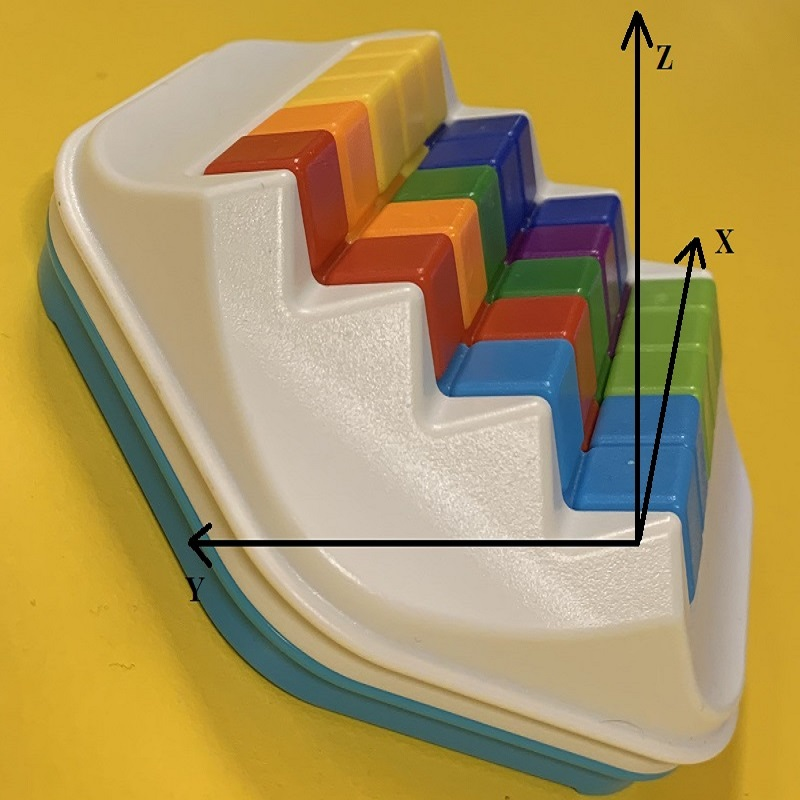
\includegraphics[width=\textwidth]{figs/ZIGZAGmodel2board.jpg}
\caption{}
\label{fig:board2A}
\end{subfigure}
\begin{subfigure}[b]{.4\textwidth}
\centering
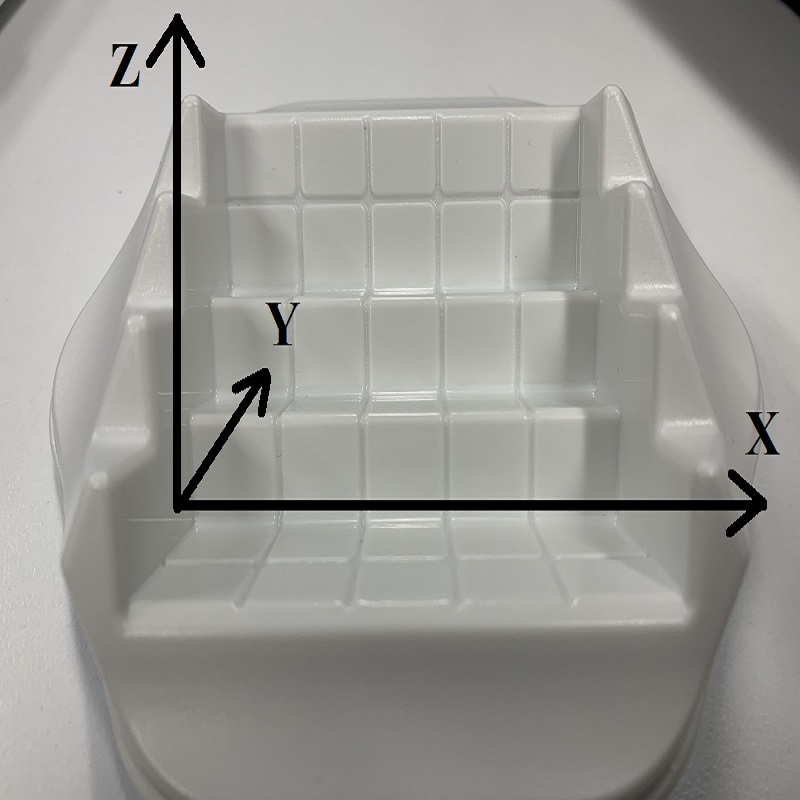
\includegraphics[width=\textwidth]{figs/3Dboard2.jpg}
\caption{}
\label{fig:board2B}
\end{subfigure}
\caption{The boards of ZIA ZAG Puzzler mode2}
  \label{fig:board2}
\end{figure}
For playing mode2, Figure~\ref{fig:board2} shows that the max number for both y-axis and z-axis are 4 and x-axis is 5, which can be represented as 
\begin{equation}
\begin{aligned}
&0<x_{0}\leq5,\\
&0<y_{0}\leq4,\\
&0<z_{0}\leq4.
\end{aligned}
\end{equation}
In addition, the board is similar to stairs, so we can get
\begin{equation}
y_{0}=z_{0}.
\end{equation}
Besides the part that is similar to stairs, the left space satisfy 
\begin{equation}
y_{0}=z_{0}+1,
\end{equation}
except when $z_{0}=4$.
Therefore, the domain of playing mode2 is
\begin{equation}
\begin{aligned}
&\forall v \in \VUnits,\\
&D(v)=\{(x,y,z) \in \mathbb{Z} \times \mathbb{Z}	\times \mathbb{Z} \mid  0<x \leq 5 , \hspace{1ex} 0<y \leq 4,\hspace{1ex} 0<z \leq 4,y=z\} \hspace{1ex}\cup\\
&\{(x,y,z) \in \mathbb{Z} \times \mathbb{Z}	\times \mathbb{Z} \mid  0<x \leq 5, \hspace{1ex} 0<y \leq 4,\hspace{1ex} 0<z \leq 3,y=z+1\}.
\end{aligned}
\end{equation}
\subsection{3D Rotation Matrix}
\label{section:3Drotationmatrix}
Tobias and Krantz \cite{r9} indicate that 3D rotations can be separately represented by rotation around x-axis, y-axis, and z-axis 
\begin{equation}
\label{equation:3Dmatrix1}
\begin{aligned}
R_{x}(\theta)=\begin{bmatrix}
1&          0&          0\\
0&\cos\theta & -\sin\theta\\
0&\sin\theta & \cos\theta\\
\end{bmatrix},
\\R_{y}(\theta)=\begin{bmatrix}
  \cos\theta&          0&\sin\theta\\
           0&          1& 0\\
-\sin\theta &          0&\cos\theta\\
\end{bmatrix},
\\R_{z}(\theta)=\begin{bmatrix}
\cos\theta&-\sin\theta&0\\
\sin\theta& \cos\theta&0\\
         0&          0&1\\
\end{bmatrix},
\end{aligned}
\end{equation}
where $R_{x}(\theta)$ is corresponding to rotation around x-axis by $\theta$, $R_{y}(\theta)$ is corresponding to the rotation around y-axis by $\theta$ and $R_{z}(\theta)$ is corresponding to the rotation around z-axis by $\theta$. Then, the combinations of the three matrix in equation~\ref{equation:3Dmatrix1} can be represented as
\begin{equation}
\begin{aligned}
&R=R_{z}(\alpha)R_{y}(\beta)R_{x}(\gamma)=\\
&\begin{bmatrix}
\cos\alpha\cos\beta&\cos\alpha\sin\beta\sin\gamma-\sin\alpha\cos\gamma&\cos\alpha\sin\beta\cos\gamma+\sin\alpha\sin\gamma\\
\sin\alpha\cos\beta&\sin\alpha\sin\beta\sin\gamma+\cos\alpha\cos\gamma&\sin\alpha\sin\beta\cos\gamma-\cos\alpha\sin\gamma\\
         -\sin\beta&                               \cos\beta\sin\gamma&\cos\beta\cos\gamma\\
\end{bmatrix}.
\end{aligned}
\end{equation}
Compared with the 2D rotation matrix, the 3D rotation matrices will consider more planes. But there are still some similarities. For example,
\begin{equation}
\label{equation:formula2}
\begin{aligned}
&x'=x\cos\theta-y\sin\theta,\\ 
&y'=x\sin\theta+y\cos\theta,\\
&z'=z,
\end{aligned}
\end{equation}
can be derived from
\begin{equation}
\begin{bmatrix}
x'\\
y'\\
z'\\
\end{bmatrix}
=R_{z}(\theta)
\begin{bmatrix}
x\\
y\\
z\\
\end{bmatrix}
\end{equation}
The forms of the $x'$ and the $y'$ in equation~\ref{equation:formula2} are the same with equation~\ref{equation:formula1}, the only difference is that this formula takes Z into account. In addition, the mirroring operation in 2D can be seen as a special case of 3D rotation. It corresponds to rotating around the xz-plane 180 degrees because 
\begin{equation}
\begin{aligned}
&x'=-x,\\
&y'=-y,\\
&z'=-z
\end{aligned}
\end{equation}
can be derived from 
\begin{equation}
\begin{bmatrix}
x'\\
y'\\
z'\\
\end{bmatrix}
=R_{y}(180^{\circ})
\begin{bmatrix}
x\\
y\\
z\\
\end{bmatrix},
\end{equation}
and $z$ will be ignored in the 2D rotation.\\
In our case, we only consider 90, 180 and 270 degrees rotations for each plane. If we separately consider each plane. There should be 4 configurations for each plane. For example, $\theta=0^{\circ}, 90^{\circ}, 180^{\circ}, 270^{\circ}$ in (3.8) is corresponding to the xy-plane. Similarly, the yz-plane and xz-plane can get 4 configurations each. Then we combine all of them, there should be 64 configurations ($4\times 4 \times 4$). However, there are only 24 configurations because of the "singularity" of Euler angles set, the geometric singularity will appear when $\beta=\pm90^{\circ}$ 
as well as $\beta=0^{\circ}$ or $180^{\circ}$ \cite{r17}. Now we consider $\beta=\pm90^{\circ}$. If $\beta=90^{\circ}$, we get 
\begin{equation}
R_{\beta=90}=R_{z}(\alpha)R_{y}(90^{\circ})R_{x}(\gamma)=
\begin{bmatrix}
0&-\sin(\alpha-\gamma)&\cos(\alpha-\gamma)\\
0&\cos(\alpha-\gamma)&\sin(\alpha-\gamma)\\
         -1&                              0&0\\
\end{bmatrix}.
\end{equation}
And when $\beta=-90^{\circ}$, it can be seen as $\beta=270^{\circ}$ because of the periodicity, we can get 
\begin{equation}
R_{\beta=270}=R_{z}(\alpha)R_{y}(270^{\circ})R_{x}(\gamma)=
\begin{bmatrix}
0&-\sin(\alpha+\gamma)&-\cos(\alpha+\gamma)\\
0&\cos(\alpha+\gamma)&-\sin(\alpha+\gamma)\\
1&                               0&0
\end{bmatrix}.
\end{equation}
Based on the formula
\begin{equation}
\begin{bmatrix}
x'\\
y'\\
z'\\
\end{bmatrix}
=R
\begin{bmatrix}
x\\
y\\
z\\
\end{bmatrix},
\end{equation}
for $\beta=90^{\circ}$,
\begin{equation}
\begin{aligned}
&x'=-y\sin(\alpha-\gamma)-z\cos(\alpha-\gamma), \\
&y'=y\cos(\alpha-\gamma)+z\sin(\alpha-\gamma), \\
&z'=-x. 
\end{aligned}
\end{equation}
and for $\beta=270^{\circ}$, 
\begin{equation}
\begin{aligned}
&x'=-y\sin(\alpha+\gamma)-z\cos(\alpha+\gamma), \\
&y'=y\cos(\alpha+\gamma)-z\sin(\alpha+\gamma), \\
&z'=x.
\end{aligned}
\end{equation}
Because in our case, the domains of both $\alpha$ and $\gamma$ are $0^{\circ}$, $90^{\circ}$, $180^{\circ}$, $270^{\circ}$ and the period of the trigonometric function is $360^{\circ}$. For (3.14), the 4 configurations are $\alpha-\gamma$=$0^{\circ}$ or $90^{\circ}$ or $180^{\circ}$ or $270^{\circ}$. For (3.15), the 4 configurations are $\alpha+\gamma$=$0^{\circ}$ or $90^{\circ}$ or $180^{\circ}$ or $270^{\circ}$.
Therefore, these 2 groups of formulas represent that there are only 4 configurations for each of them. In other words, the separated $\alpha$ and $\gamma$ are meaningless. What we should consider is $\alpha-\gamma$ for (3.14) and $\alpha+\gamma$ for (3.15). For (3.14), we assign 0,90,180 and 270 degrees to the $(\alpha-\gamma)$, we get
\begin{itemize}
  \item  $x'=-y\sin(0^{\circ})-z\cos(0^{\circ}),\hspace{5pt} y'=y\cos(0^{\circ})+z\sin(0^{\circ}),\hspace{5pt} z'=-x \\\implies x'=-z,\hspace{5pt} y'=y,\hspace{5pt} z'=-x$,
  \item  $x'=-y\sin(90^{\circ})-z\cos(90^{\circ}), \hspace{5pt} y'=y\cos(90^{\circ})+z\sin(90^{\circ}), \hspace{5pt} z'=-x\\\implies x'=-y,\hspace{5pt} y'=z,\hspace{5pt} z'=-x$,
  \item  $x'=-y\sin(180^{\circ})-z\cos(180^{\circ}), \hspace{5pt} y'=y\cos(180^{\circ})+z\sin(180^{\circ}), \hspace{5pt} z'=-x\\\implies x'=z,\hspace{5pt} y'=-y,\hspace{5pt} z'=-x$,
  \item  $x'=-y\sin(270^{\circ})-z\cos(270^{\circ}), \hspace{5pt} y'=y\cos(270^{\circ})+z\sin(270^{\circ}), \hspace{5pt} z'=-x\\\implies x'=y, \hspace{5pt}y'=-z,\hspace{5pt} z'=-x$.
  \label{3Drotation24situations1}
\end{itemize}
For (3.15), we assign 0,90,180 and 270 degrees to the $(\alpha+\gamma)$, we get
\begin{itemize}
  \item  $x'=-y\sin(0^{\circ})-z\cos(0^{\circ}),\hspace{5pt} y'=y\cos(0^{\circ})-z\sin(0^{\circ}),\hspace{5pt} z'=-x \\\implies x'=-z,\hspace{5pt} y'=y,\hspace{5pt} z'=x$,
  \item  $x'=-y\sin(90^{\circ})-z\cos(90^{\circ}),\hspace{5pt} y'=y\cos(90^{\circ})-z\sin(90^{\circ}),\hspace{5pt} z'=-x\\\implies x'=-y,\hspace{5pt} y'=-z,\hspace{5pt} z'=x$,
  \item  $x'=-y\sin(180^{\circ})-z\cos(180^{\circ}),\hspace{5pt} y'=y\cos(180^{\circ})-z\sin(180^{\circ}),\hspace{5pt} z'=-x\\\implies x'=z,\hspace{5pt} y'=-y,\hspace{5pt} z'=x$,
  \item  $x'=-y\sin(270^{\circ})-z\cos(270^{\circ}),\hspace{5pt} y'=y\cos(270^{\circ})-z\sin(270^{\circ}),\hspace{5pt} z'=-x\\\implies x'=y, \hspace{5pt}y'=z,\hspace{5pt} z'=x$.
  \label{3Drotation24situations2}
\end{itemize}
Then, we consider  $\beta=0^{\circ}$ and $\beta=180^{\circ}$. Based on (3.6), when $\beta=0^{\circ}$, we get
\begin{equation}
R=R_{z}(\alpha)R_{y}(0^{\circ})R_{x}(\gamma)=
\begin{bmatrix}
\cos\alpha&-\sin\alpha\cos\gamma&\sin\alpha\sin\gamma\\
\sin\alpha&\cos\alpha\cos\gamma&-\cos\alpha\sin\gamma\\
0&          \sin\gamma&\cos\gamma\\
\end{bmatrix}.
\end{equation}
When $\beta=180^{\circ}$, we get
\begin{equation}
R=R_{z}(\alpha)R_{y}(180^{\circ})R_{x}(\gamma)=
\begin{bmatrix}
-\cos\alpha&-\sin\alpha\cos\gamma&\sin\alpha\sin\gamma\\
-\sin\alpha&\cos\alpha\cos\gamma&-\cos\alpha\sin\gamma\\
0&                               -\sin\gamma&-\cos\gamma\\
\end{bmatrix}.
\end{equation}
In (3.17), we assign $\alpha=\alpha+180^{\circ}$ and $\gamma=\gamma+180^{\circ}$, then it change to
\begin{equation}
\begin{aligned}
&R=R_{z}(\alpha+180^{\circ})R_{y}(180^{\circ})R_{x}(\gamma+180^{\circ})=\\
&\begin{bmatrix}
-\cos(\alpha+180^{\circ})&-\sin(\alpha+180^{\circ})\cos(\gamma+180^{\circ})&\sin(\alpha+180^{\circ})\sin(\gamma+180^{\circ})\\
-\sin(\alpha+180^{\circ})&\cos(\alpha+180^{\circ})\cos(\gamma+180^{\circ})&-\cos(\alpha+180^{\circ})\sin(\gamma+180^{\circ})\\
0&                               -\sin(\gamma+180^{\circ})&-\cos(\gamma+180^{\circ})
\end{bmatrix}\\
&=\begin{bmatrix}
\cos(\alpha)&-\sin(\alpha)\cos(\gamma)&\sin(\alpha)\sin(\gamma)\\
\sin(\alpha)&\cos(\alpha)\cos(\gamma)&-\cos(\alpha)\sin(\gamma)\\
0&                               \sin(\gamma)&\cos(\gamma)\\
\end{bmatrix}.
\end{aligned}
\end{equation}
Therefore, based on (3.16) and (3.18),
\begin{equation}
R_{z}(\alpha)R_{y}(0^{\circ})R_{x}(\gamma)=R_{z}(\alpha+180^{\circ})R_{y}(180^{\circ})R_{x}(\gamma+180^{\circ})
\end{equation}, 
which means that when $\beta=0^{\circ}$, regardless of the number of degrees of $\alpha$ and the number of degrees of $\gamma$, there are always corresponding $\alpha+180^{\circ}$, $\gamma+180^{\circ}$ when $\beta=180^{\circ}$. Even though the number of degrees of $\alpha+180^{\circ}$ or $\gamma+180^{\circ}$ may be more than $360^{\circ}$, it can always find a corresponding from $0^{\circ}$ to $360^{\circ}$ according to the periodicity of trigonometric function. For example, \begin{equation}
\begin{aligned}
&\circled{1}R_{z}(270^{\circ})Ry(0^{\circ})R_{x}(270^{\circ}) = R_{z}(450^{\circ})R_{y}(180^{\circ})R_{x}(450^{\circ})\\ 
&\circled{2}R_{z}(450^{\circ})Ry(180^{\circ})R_{x}(450^{\circ}) = R_{z}(90^{\circ})R_{y}(180^{\circ})R_{x}(90^{\circ})\\
&\circled{1},\circled{2}\implies R_{z}(270^{\circ})Ry(0^{\circ})R_{x}(270^{\circ})   = R_{z}(90^{\circ})R_{y}(180^{\circ})R_{x}(90^{\circ}).
\end{aligned}
\end{equation}
Hence, all combinations among $\beta=0^{\circ}$, $\theta=0^{\circ}$ or $90^{\circ}$ or $180^{\circ}$ or $270^{\circ}$ and $\gamma=0^{\circ}$ or $90^{\circ}$ or $180^{\circ}$ or $270^{\circ}$ can be obtained from one combination among $\beta=180^{\circ}$, $\theta=0^{\circ}$ or $90^{\circ}$ or $180^{\circ}$ or $270^{\circ}$ and $\gamma=0^{\circ}$ or $90^{\circ}$ or $180^{\circ}$ or $270^{\circ}$. So we only need to consider the all configurations when $\beta=0^{\circ}$ because the all configurations in $\beta=180^{\circ}$ are duplicates. For (3.16) we assign $\theta=0^{\circ},\gamma=0^{\circ}$, $\theta=0^{\circ},\gamma=90^{\circ}$,...,$\theta=270^{\circ},\gamma=180^{\circ}$, $\theta=270^{\circ},\gamma=270^{\circ}$. we get
\begin{itemize}
  \item  $x'=x$,   $y'=y$,    $z'=z$,
  \item  $x'=x$,   $y'=-z$,   $z'=y$, 
  \item  $x'=x$,   $y'=-y$,   $z'=-z$, 
  \item  $x'=x$,   $y'=z$,    $z'=-y$,
  \item  $x'=-y$,  $y'=x$,    $z'=z$,
  \item  $x'=z$,   $y'=x$,    $z'=y$,
  \item  $x'=y$,   $y'=x$,    $z'=-z$,
  \item  $x'=-z$,  $y'=x$,    $z'=-y$,
  \item  $x'=-x$,  $y'=-y$,   $z'=z$,
  \item  $x'=-x$,  $y'=z$,    $z'=y$,
  \item  $x'=-x$,  $y'=y$,    $z'=-z$,
  \item  $x'=-x$,  $y'=-z$,   $z'=-y$,
  \item  $x'=y$,   $y'=-x$,   $z'=z$,
  \item  $x'=-z$,  $y'=-x$,   $z'=y$,
  \item  $x'=-y$,  $y'=-x$,   $z'=-z$,
  \item  $x'=z$,   $y'=-x$,   $z'=-y$.
  \label{3Drotation24situations3}
\end{itemize}
There should be a total of 16 configurations (4$\times$4). Finally, consider the all configurations in $\beta=90^{\circ}$,$\beta=270^{\circ}$,$\beta=^{\circ}0$ and $\beta=180^{\circ}$. There should be a total of 4+4+16=24 configurations.
\subsection{Constraints}
\begin{figure}[htbp]
\centering
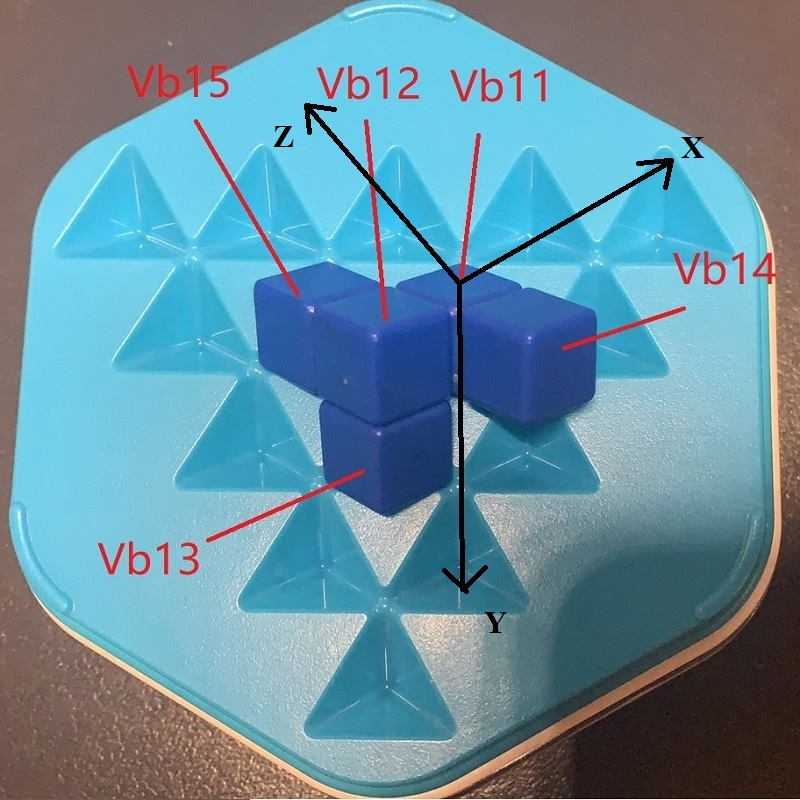
\includegraphics[width=0.5\textwidth]{figs/3Drotateexplain.jpg}
\caption{3Dblue1 initial state}
\label{fig:3Dblue1explanation}
\end{figure}
As is shown in Figure~\ref{fig:3Dblue1explanation}, the unit which is corresponding to the first variable ($V_{b11}$) will be considered as a point $(x,y,z)$. Therefore, the $V_{b11}$, $V_{b12}$, $V_{b13}$, $V_{b14}$ and $V_{b15}$ are respectively represented as $(x,y,z)$, $(x-1,y,z)$, $(x-1,y+1,z)$, $(x,y,z-1)$ and $(x-1,y,z+1)$, which indicate that all other variables are connection with the first variables. Similar to 2D rotation, the basic idea of 3D rotation is all other units of pieces rotate around the first unit of pieces. According to chapter~\ref{section:3Drotationmatrix}, there are 24 rotation configurations. So we get
\begin{equation}\tiny
\begin{aligned}
&\Cons{b11}{b12}{b13}{b14}{b15}=\{((x_{1},y_{1},z_{1}),(x_{2},y_{2},z_{2}),(x_{3},y_{3},z_{3}),(x_{4},y_{4},z_{4}),(x_{5},y_{5},z_{5}))\in \\
&\Domain {b11} \times \Domain{b12}\times \Domain{b13}\times \Domain{b14}\times \Domain{b15} \mid\\
&(x_{2}=x_{1}-1,\hspace{1ex} y_{2}=y_{1},\hspace{1ex} z_{2}=z_{1},\hspace{1ex} x_{3}=x_{1}-1,\hspace{1ex} y_{3}=y_{1}+1,\hspace{1ex} z_{3}=z_{1},\hspace{1ex} x_{4}=x_{1},\\
&\hspace{1ex} y_{4}=y_{1},\hspace{1ex} z_{4}=z_{1}-1,\hspace{1ex} x_{5}=x_{1}-1,\hspace{1ex} y_{5}=y_{1},\hspace{1ex} z_{5}=z_{1}+1)&or\\ 
&(x_{2}=x_{1},\hspace{1ex} y_{2}=y_{1}+1,\hspace{1ex} z_{2}=z_{1},\hspace{1ex} x_{3}=x_{1},\hspace{1ex} y_{3}=y_{1}+1,\hspace{1ex} z_{3}=z_{1}-1,\hspace{1ex} x_{4}=x_{1}-1,\\
&\hspace{1ex} y_{4}=y_{1},\hspace{1ex} z_{4}=z_{1},\hspace{1ex} x_{5}=x_{1}+1,\hspace{1ex} y_{5}=y_{1}+1,\hspace{1ex} z_{5}=z_{1})&or\\ 
&(x_{2}=x_{1},\hspace{1ex} y_{2}=y_{1}+1,\hspace{1ex} z_{2}=z_{1},\hspace{1ex} x_{3}=x_{1},\hspace{1ex} y_{3}=y_{1}+1,\hspace{1ex} z_{3}=z_{1}+1,\hspace{1ex} x_{4}=x_{1}+1,\\
&\hspace{1ex} y_{4}=y_{1},\hspace{1ex} z_{4}=z_{1},\hspace{1ex} x_{5}=x_{1}-1,\hspace{1ex} y_{5}=y_{1}+1,\hspace{1ex} z_{5}=z_{1})&or\\ 
&(x_{2}=x_{1},\hspace{1ex} y_{2}=y_{1},\hspace{1ex} z_{2}=z_{1}-1,\hspace{1ex} x_{3}=x_{1}-1,\hspace{1ex} y_{3}=y_{1},\hspace{1ex} z_{3}=z_{1}-1,\hspace{1ex} x_{4}=x_{1},\\
&\hspace{1ex} y_{4}=y_{1}+1,\hspace{1ex} z_{4}=z_{1},\hspace{1ex} x_{5}=x_{1},\hspace{1ex} y_{5}=y_{1}-1,\hspace{1ex} z_{5}=z_{1}-1)&or\\ 
&(x_{2}=x_{1}-1,\hspace{1ex} y_{2}=y_{1},\hspace{1ex} z_{2}=z_{1},\hspace{1ex} x_{3}=x_{1}-1,\hspace{1ex} y_{3}=y_{1}-1,\hspace{1ex} z_{3}=z_{1},\hspace{1ex} x_{4}=x_{1},\\
&\hspace{1ex} y_{4}=y_{1},\hspace{1ex} z_{4}=z_{1}+1,\hspace{1ex} x_{5}=x_{1}-1,\hspace{1ex} y_{5}=y_{1},\hspace{1ex} z_{5}=z_{1}-1)&or\\ 
&(x_{2}=x_{1}+1,\hspace{1ex} y_{2}=y_{1},\hspace{1ex} z_{2}=z_{1},\hspace{1ex} x_{3}=x_{1}+1,\hspace{1ex} y_{3}=y_{1}-1,\hspace{1ex} z_{3}=z_{1},\hspace{1ex} x_{4}=x_{1},\\
&\hspace{1ex} y_{4}=y_{1},\hspace{1ex} z_{4}=z_{1}-1,\hspace{1ex} x_{5}=x_{1}+1,\hspace{1ex} y_{5}=y_{1},\hspace{1ex} z_{5}=z_{1}+1)&or\\ 
&(x_{2}=x_{1},\hspace{1ex} y_{2}=y_{1}-1,\hspace{1ex} z_{2}=z_{1},\hspace{1ex} x_{3}=x_{1},\hspace{1ex} y_{3}=y_{1}-1,\hspace{1ex} z_{3}=z_{1}-1,\hspace{1ex} x_{4}=x_{1}+1,\\
&\hspace{1ex} y_{4}=y_{1},\hspace{1ex} z_{4}=z_{1},\hspace{1ex} x_{5}=x_{1}-1,\hspace{1ex} y_{5}=y_{1}-1,\hspace{1ex} z_{5}=z_{1})&or\\ 
&(x_{2}=x_{1},\hspace{1ex} y_{2}=y_{1}-1,\hspace{1ex} z_{2}=z_{1},\hspace{1ex} x_{3}=x_{1},\hspace{1ex} y_{3}=y_{1}-1,\hspace{1ex} z_{3}=z_{1}+1,\hspace{1ex} x_{4}=x_{1}-1,\\
&\hspace{1ex} y_{4}=y_{1},\hspace{1ex} z_{4}=z_{1},\hspace{1ex} x_{5}=x_{1}+1,\hspace{1ex} y_{5}=y_{1}-1,\hspace{1ex} z_{5}=z_{1})&or\\ 
&(x_{2}=x_{1},\hspace{1ex} y_{2}=y_{1}+1,\hspace{1ex} z_{2}=z_{1},\hspace{1ex} x_{3}=x_{1}+1,\hspace{1ex} y_{3}=y_{1}+1,\hspace{1ex} z_{3}=z_{1},\hspace{1ex} x_{4}=x_{1},\\
&\hspace{1ex} y_{4}=y_{1},\hspace{1ex} z_{4}=z_{1}-1,\hspace{1ex} x_{5}=x_{1},\hspace{1ex} y_{5}=y_{1}+1,\hspace{1ex} z_{5}=z_{1}+1)&or\\ 
&(x_{2}=x_{1},\hspace{1ex} y_{2}=y_{1},\hspace{1ex} z_{2}=z_{1}+1,\hspace{1ex} x_{3}=x_{1},\hspace{1ex} y_{3}=y_{1}-1,\hspace{1ex} z_{3}=z_{1}+1,\hspace{1ex} x_{4}=x_{1}+1,\\
&\hspace{1ex} y_{4}=y_{1},\hspace{1ex} z_{4}=z_{1},\hspace{1ex} x_{5}=x_{1}-1,\hspace{1ex} y_{5}=y_{1},\hspace{1ex} z_{5}=z_{1}+1)&or\\ 
&(x_{2}=x_{1},\hspace{1ex} y_{2}=y_{1},\hspace{1ex} z_{2}=z_{1}+1,\hspace{1ex} x_{3}=x_{1}+1,\hspace{1ex} y_{3}=y_{1},\hspace{1ex} z_{3}=z_{1}+1,\hspace{1ex} x_{4}=x_{1},\\
&\hspace{1ex} y_{4}=y_{1}+1,\hspace{1ex} z_{4}=z_{1},\hspace{1ex} x_{5}=x_{1},\hspace{1ex} y_{5}=y_{1}-1,\hspace{1ex} z_{5}=z_{1}+1)&or\\ 
&(x_{2}=x_{1},\hspace{1ex} y_{2}=y_{1},\hspace{1ex} z_{2}=z_{1}-1,\hspace{1ex} x_{3}=x_{1},\hspace{1ex} y_{3}=y_{1}+1,\hspace{1ex} z_{3}=z_{1}-1,\hspace{1ex} x_{4}=x_{1}+1,\\
&\hspace{1ex} y_{4}=y_{1},\hspace{1ex} z_{4}=z_{1},\hspace{1ex} x_{5}=x_{1}-1,\hspace{1ex} y_{5}=y_{1},\hspace{1ex} z_{5}=z_{1}-1)&or\\ 
&(x_{2}=x_{1},\hspace{1ex} y_{2}=y_{1}-1,\hspace{1ex} z_{2}=z_{1},\hspace{1ex} x_{3}=x_{1}-1,\hspace{1ex} y_{3}=y_{1}-1,\hspace{1ex} z_{3}=z_{1},\hspace{1ex} x_{4}=x_{1},\\
&\hspace{1ex} y_{4}=y_{1},\hspace{1ex} z_{4}=z_{1}-1,\hspace{1ex} x_{5}=x_{1},\hspace{1ex} y_{5}=y_{1}-1,\hspace{1ex} z_{5}=z_{1}+1)&or\\ 
&(x_{2}=x_{1}+1,\hspace{1ex} y_{2}=y_{1},\hspace{1ex} z_{2}=z_{1},\hspace{1ex} x_{3}=x_{1}+1,\hspace{1ex} y_{3}=y_{1},\hspace{1ex} z_{3}=z_{1}-1,\hspace{1ex} x_{4}=x_{1},\\
&\hspace{1ex} y_{4}=y_{1}+1,\hspace{1ex} z_{4}=z_{1},\hspace{1ex} x_{5}=x_{1}+1,\hspace{1ex} y_{5}=y_{1}-1,\hspace{1ex} z_{5}=z_{1})&or\\
&(x_{2}=x_{1}+1,\hspace{1ex} y_{2}=y_{1},\hspace{1ex} z_{2}=z_{1},\hspace{1ex} x_{3}=x_{1}+1,\hspace{1ex} y_{3}=y_{1}+1,\hspace{1ex} z_{3}=z_{1},\hspace{1ex} x_{4}=x_{1},\\
&\hspace{1ex} y_{4}=y_{1},\hspace{1ex} z_{4}=z_{1}+1,\hspace{1ex} x_{5}=x_{1}+1,\hspace{1ex} y_{5}=y_{1},\hspace{1ex} z_{5}=z_{1}-1)&or\\ 
&(x_{2}=x_{1},\hspace{1ex} y_{2}=y_{1},\hspace{1ex} z_{2}=z_{1}-1,\hspace{1ex} x_{3}=x_{1},\hspace{1ex} y_{3}=y_{1}-1,\hspace{1ex} z_{3}=z_{1}-1,\hspace{1ex} x_{4}=x_{1}-1,\\
&\hspace{1ex} y_{4}=y_{1},\hspace{1ex} z_{4}=z_{1},\hspace{1ex} x_{5}=x_{1}+1,\hspace{1ex} y_{5}=y_{1},\hspace{1ex} z_{5}=z_{1}-1)&or\\ 
&(x_{2}=x_{1},\hspace{1ex} y_{2}=y_{1},\hspace{1ex} z_{2}=z_{1}+1,\hspace{1ex} x_{3}=x_{1},\hspace{1ex} y_{3}=y_{1}+1,\hspace{1ex} z_{3}=z_{1}+1,\hspace{1ex} x_{4}=x_{1}-1,\\
&\hspace{1ex} y_{4}=y_{1},\hspace{1ex} z_{4}=z_{1},\hspace{1ex} x_{5}=x_{1}+1,\hspace{1ex} y_{5}=y_{1},\hspace{1ex} z_{5}=z_{1}+1)&or\\ 
&(x_{2}=x_{1},\hspace{1ex} y_{2}=y_{1},\hspace{1ex} z_{2}=z_{1}-1,\hspace{1ex} x_{3}=x_{1}+1,\hspace{1ex} y_{3}=y_{1},\hspace{1ex} z_{3}=z_{1}-1,\hspace{1ex} x_{4}=x_{1},\\
&\hspace{1ex} y_{4}=y_{1}-1,\hspace{1ex} z_{4}=z_{1},\hspace{1ex} x_{5}=x_{1},\hspace{1ex} y_{5}=y_{1}+1,\hspace{1ex} z_{5}=z_{1}-1)&or\\ 
&(x_{2}=x_{1},\hspace{1ex} y_{2}=y_{1}-1,\hspace{1ex} z_{2}=z_{1},\hspace{1ex} x_{3}=x_{1}+1,\hspace{1ex} y_{3}=y_{1}-1,\hspace{1ex} z_{3}=z_{1},\hspace{1ex} x_{4}=x_{1},\\
&\hspace{1ex} y_{4}=y_{1},\hspace{1ex} z_{4}=z_{1}+1,\hspace{1ex} x_{5}=x_{1},\hspace{1ex} y_{5}=y_{1}-1,\hspace{1ex} z_{5}=z_{1}-1)&or\\ 
&(x_{2}=x_{1},\hspace{1ex} y_{2}=y_{1}+1,\hspace{1ex} z_{2}=z_{1},\hspace{1ex} x_{3}=x_{1}-1,\hspace{1ex} y_{3}=y_{1}+1,\hspace{1ex} z_{3}=z_{1},\hspace{1ex} x_{4}=x_{1},\\
&\hspace{1ex} y_{4}=y_{1},\hspace{1ex} z_{4}=z_{1}+1,\hspace{1ex} x_{5}=x_{1},\hspace{1ex} y_{5}=y_{1}+1,\hspace{1ex} z_{5}=z_{1}-1)&or\\ 
&(x_{2}=x_{1}+1,\hspace{1ex} y_{2}=y_{1},\hspace{1ex} z_{2}=z_{1},\hspace{1ex} x_{3}=x_{1}+1,\hspace{1ex} y_{3}=y_{1},\hspace{1ex} z_{3}=z_{1}+1,\hspace{1ex} x_{4}=x_{1},\\
&\hspace{1ex} y_{4}=y_{1}-1,\hspace{1ex} z_{4}=z_{1},\hspace{1ex} x_{5}=x_{1}+1,\hspace{1ex} y_{5}=y_{1}+1,\hspace{1ex} z_{5}=z_{1})&or\\ 
&(x_{2}=x_{1}-1,\hspace{1ex} y_{2}=y_{1},\hspace{1ex} z_{2}=z_{1},\hspace{1ex} x_{3}=x_{1}-1,\hspace{1ex} y_{3}=y_{1},\hspace{1ex} z_{3}=z_{1}+1,\hspace{1ex} x_{4}=x_{1},\\
&\hspace{1ex} y_{4}=y_{1}+1,\hspace{1ex} z_{4}=z_{1},\hspace{1ex} x_{5}=x_{1}-1,\hspace{1ex} y_{5}=y_{1}-1,\hspace{1ex} z_{5}=z_{1})&or\\ 
&(x_{2}=x_{1},\hspace{1ex} y_{2}=y_{1},\hspace{1ex} z_{2}=z_{1}+1,\hspace{1ex} x_{3}=x_{1}-1,\hspace{1ex} y_{3}=y_{1},\hspace{1ex} z_{3}=z_{1}+1,\hspace{1ex} x_{4}=x_{1},\\
&\hspace{1ex} y_{4}=y_{1}-1,\hspace{1ex} z_{4}=z_{1},\hspace{1ex} x_{5}=x_{1},\hspace{1ex} y_{5}=y_{1}+1,\hspace{1ex} z_{5}=z_{1}+1)&or\\ 
&(x_{2}=x_{1}-1,\hspace{1ex} y_{2}=y_{1},\hspace{1ex} z_{2}=z_{1},\hspace{1ex} x_{3}=x_{1}-1,\hspace{1ex} y_{3}=y_{1},\hspace{1ex} z_{3}=z_{1}-1,\hspace{1ex} x_{4}=x_{1},\\
&\hspace{1ex} y_{4}=y_{1}-1,\hspace{1ex} z_{4}=z_{1},\hspace{1ex} x_{5}=x_{1}-1,\hspace{1ex} y_{5}=y_{1}+1,\hspace{1ex} z_{5}=z_{1})\}.
Similarly, we can get the constraints for other pieces.
\end{aligned}
\end{equation}